\documentclass[11pt,a4paper]{article}

\usepackage[utf8]{inputenc}
\usepackage[T1]{fontenc}
\usepackage{lmodern}
\usepackage[margin=2.5cm]{geometry}
\usepackage{graphicx}
\usepackage{booktabs}
\usepackage{multirow}
\usepackage{xcolor}
\usepackage{tikz}
\usepackage{pgfplots}
\pgfplotsset{compat=1.18}
\usepackage{amsmath}
\usepackage{siunitx}
\usepackage[font=small,labelfont=bf]{caption}
\usepackage[colorlinks=true,allcolors=blue!55!black]{hyperref}

\sisetup{detect-all, separate-uncertainty}

% A box for claims that are provisional, so the reader cannot miss them.
\usepackage{mdframed}
\newmdenv[
  linecolor=red!55!black, linewidth=0.8pt,
  backgroundcolor=red!3,
  innertopmargin=6pt, innerbottommargin=6pt,
  skipabove=8pt, skipbelow=8pt
]{caveat}

\title{\textbf{Initial structural findings on aRES}\\[2pt]
       \large Domain architecture and an N-terminal Zn(Cys)$_4$ ribbon}
\author{}
\date{\today}

\begin{document}
\maketitle
\vspace{-2.2em}

%===============================================================
\section*{Summary}
\addcontentsline{toc}{section}{Summary}

Four findings, in descending order of how well they are supported.

\begin{enumerate}\itemsep3pt
\item \textbf{aRES carries a Zn(Cys)$_4$ ribbon at its N-terminus} (C8, C11, C31,
      C34; CxxC\,$\dots$\,CxxC). The coordination geometry is quantitatively
      tetrahedral and the model is confident there (pLDDT 90.8). This is a
      structural zinc site, not a disulfide cluster.
\item \textbf{The N-terminal block is bimodular}, and this resolves a standing
      disagreement between the structural and the Pfam annotation: Pfam's
      PF18870 call begins at residue 49, which is \emph{exactly} where the zinc
      ribbon ends. The two annotations are not in conflict --- Pfam is blind to
      the ribbon.
\item \textbf{The architecture is extended, with a real hinge at 121--125}
      ($R_g = \SI{31.9}{\angstrom}$; block centroids \SI{50.5}{\angstrom} apart;
      hinge pLDDT 52.6). A compact 52\,kDa globule would be
      $\sim$\SI{25}{\angstrom}.
\item \textbf{The recognition interface remains open.} A single cofold places
      the phage escape residue against NTD-1, but at poor ipTM. It is a lead,
      not a result; \S\ref{sec:recognition} states plainly what it does and does
      not support.
\end{enumerate}

%===============================================================
\section{Domain architecture}
\label{sec:domains}

Two independent annotations of aRES disagree, and the disagreement is
informative rather than a nuisance (Fig.~\ref{fig:map}).

\begin{table}[htbp]
\centering
\caption{Domain boundaries from the two annotation routes. Mean pLDDT is the
per-region mean over the \texttt{aRES\_Zn\_segA} monomer model
(residues 1--447).}
\label{tab:domains}
\small
\begin{tabular}{llcl}
\toprule
\textbf{Region} & \textbf{Residues} & \textbf{mean pLDDT} & \textbf{Source} \\
\midrule
Zn ribbon            & 1--48    & 84.9 & AF3 PAE block; this work \\
NTD-1                & 49--120  & 80.9 & AF3 PAE block \\
Hinge                & 121--125 & \textbf{52.6} & AF3 PAE \\
RES block            & 126--447 & 78.0 & AF3 PAE block \\
\quad flexible loop  & 392--408 & \textbf{48.1} & internal; not trimmable \\
C-terminal tail      & 448--459 & \textbf{53.9} & MobiDB disorder \\
\midrule
PF18870 (NTD-1)      & 49--136  & ---  & InterPro \\
PF08808 (RES)        & 199--363 & ---  & InterPro \\
\bottomrule
\end{tabular}
\end{table}

\begin{figure}[htbp]
\centering
% fig_domain_map.tex -- linear domain map of aRES (UC5), two annotation tracks.
% Boundaries: docs/05 section 1.1 (PAE blocks) and docs/07 section 1 (Zn ribbon).
% Coordinates are in residue units: the x unit vector is set to 0.0295 cm.
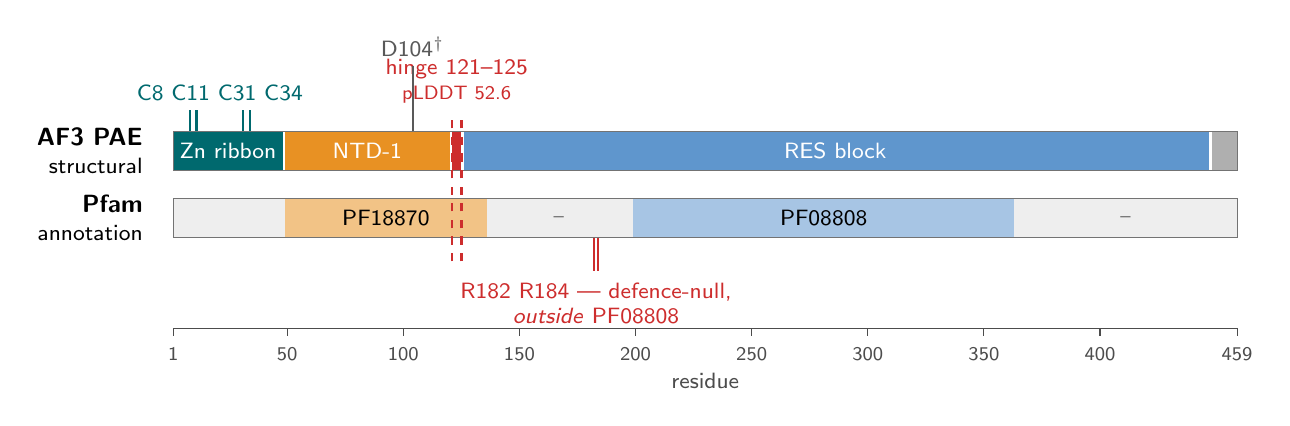
\begin{tikzpicture}[x=0.0295cm, y=1cm, font=\sffamily\small]

  \definecolor{znribbon}{RGB}{0,105,110}
  \definecolor{ntd1col}{RGB}{232,145,35}
  \definecolor{hingecol}{RGB}{205,45,45}
  \definecolor{rescol}{RGB}{95,150,205}
  \definecolor{tailcol}{RGB}{175,175,175}
  \definecolor{unassigned}{RGB}{238,238,238}

  % ---------- track 1: AF3 PAE structural blocks ----------
  \node[anchor=east, align=right] at (-8, 1.10)
    {\textbf{AF3 PAE}\\[-1pt]\footnotesize structural};

  \fill[znribbon]  (1,0.85)   rectangle (48,1.35);
  \fill[ntd1col]   (49,0.85)  rectangle (120,1.35);
  \fill[hingecol]  (121,0.85) rectangle (125,1.35);
  \fill[rescol]    (126,0.85) rectangle (447,1.35);
  \fill[tailcol]   (448,0.85) rectangle (459,1.35);
  \draw[black!55, line width=0.3pt] (1,0.85) rectangle (459,1.35);

  \node[white]        at (24.5,1.10) {\footnotesize Zn ribbon};
  \node[white]        at (84.5,1.10) {\footnotesize NTD-1};
  \node[white]        at (286,1.10)  {\footnotesize RES block};

  % ---------- track 2: Pfam ----------
  \node[anchor=east, align=right] at (-8, 0.25)
    {\textbf{Pfam}\\[-1pt]\footnotesize annotation};

  \fill[unassigned] (1,0)   rectangle (459,0.50);
  \fill[ntd1col!55] (49,0)  rectangle (136,0.50);
  \fill[rescol!55]  (199,0) rectangle (363,0.50);
  \draw[black!55, line width=0.3pt] (1,0) rectangle (459,0.50);

  \node at (92.5,0.25) {\footnotesize PF18870};
  \node at (281,0.25)  {\footnotesize PF08808};
  \node[black!55] at (167,0.25) {\scriptsize --};
  \node[black!55] at (411,0.25) {\scriptsize --};

  % ---------- the hinge discrepancy ----------
  \draw[hingecol, line width=0.9pt, dashed] (121,-0.30) -- (121,1.55);
  \draw[hingecol, line width=0.9pt, dashed] (125,-0.30) -- (125,1.55);
  \node[hingecol, anchor=south, align=center] at (123,1.58)
    {\footnotesize hinge 121--125\\[-2pt]\scriptsize pLDDT 52.6};

  % ---------- zinc-site cysteines ----------
  \foreach \r in {8,11,31,34}{%
    \draw[znribbon, line width=0.8pt] (\r,1.35) -- (\r,1.62);}
  \node[znribbon, anchor=south, align=center] at (21,1.62)
    {\footnotesize C8 C11 C31 C34};

  % ---------- D104 ----------
  \draw[black!65, line width=0.7pt] (104,1.35) -- (104,2.18);
  \node[black!65, anchor=south] at (104,2.18) {\footnotesize D104$^{\dagger}$};

  % ---------- R182 / R184 fall OUTSIDE the Pfam RES call ----------
  \foreach \r in {182,184}{%
    \draw[hingecol, line width=0.8pt] (\r,0) -- (\r,-0.42);}
  \node[hingecol, anchor=north, align=center] at (183,-0.45)
    {\footnotesize R182 R184 --- defence-null,\\[-2pt]
     \footnotesize \emph{outside} PF08808};

  % ---------- residue axis ----------
  \draw[black!70] (1,-1.15) -- (459,-1.15);
  \foreach \r in {1,50,100,150,200,250,300,350,400,459}{%
    \draw[black!70] (\r,-1.15) -- (\r,-1.25);
    \node[anchor=north, black!70] at (\r,-1.27) {\scriptsize \r};}
  \node[anchor=north, black!70] at (230,-1.60) {\footnotesize residue};

\end{tikzpicture}

\caption{\textbf{Linear domain map of aRES.} Upper track: structural blocks from
the AF3 PAE matrix. Lower track: the Pfam annotation, with unassigned regions in
grey. Two mismatches matter. \textbf{(i)} PF18870 runs to residue 136, crossing
the hinge, so a construct cut on the Pfam boundary severs a flexible joint rather
than a domain edge. \textbf{(ii)} PF08808 (199--363) \emph{excludes} R182 and
R184, both of which are defence-null --- a ``RES domain'' construct built on the
Pfam call would physically lack two active-site arginines and be inactive for a
trivial reason. $^{\dagger}$D104 is shown for orientation only; see
\S\ref{sec:recognition} for why it is not load-bearing.}
\label{fig:map}
\end{figure}

\paragraph{Why trust the PAE blocks.} The R182/R184 argument is the decisive one
and it is checkable: both residues are known to abolish defence, and both lie
outside the Pfam RES call. The PAE block 126--447 contains them. Separately, the
hinge at 121--125 scores pLDDT 52.6 against $\sim$80 on either side
(Fig.~\ref{fig:plddt}), which is independent evidence that it is a genuine
flexible joint and not a modelling artefact.

\paragraph{The remainder problem.} Coloured on Pfam boundaries, roughly a third
of aRES (137--198 and 364--459, $\sim$158 residues) falls into no annotated
domain at all. Coloured on the PAE blocks there is no unassigned remainder. This
is worth stating because the obvious first figure --- a cartoon coloured by Pfam
--- makes the protein look more fragmentary than it is.

\begin{figure}[htbp]
\centering
% fig_plddt.tex -- per-residue confidence trace of the aRES monomer model.
% Data: plddt.dat, generated from the B-factor column of aRES_Zn_segA.pdb
% (per-residue mean). That column is a pLDDT-like confidence field, verified
% against the per-region means recorded in docs/07: HIGH = confident.
\begin{tikzpicture}
\begin{axis}[
    width=0.95\textwidth, height=5.2cm,
    xlabel={residue}, ylabel={pLDDT},
    xmin=1, xmax=447, ymin=20, ymax=100,
    xtick={1,50,100,150,200,250,300,350,400,447},
    ytick={20,40,60,80,100},
    tick label style={font=\footnotesize},
    label style={font=\small},
    axis line style={black!70},
    grid=major, grid style={black!12, line width=0.3pt},
    clip mode=individual,
]

  % confidence bands
  \addplot[draw=none, fill=green!12, forget plot]
    coordinates {(1,70) (447,70) (447,100) (1,100)} \closedcycle;
  \addplot[draw=none, fill=red!10, forget plot]
    coordinates {(1,20) (447,20) (447,50) (1,50)} \closedcycle;

  % the two low-confidence regions called out in docs/07
  \addplot[draw=none, fill=red!28, forget plot]
    coordinates {(121,20) (125,20) (125,100) (121,100)} \closedcycle;
  \addplot[draw=none, fill=orange!22, forget plot]
    coordinates {(392,20) (408,20) (408,100) (392,100)} \closedcycle;

  \addplot[black!80, line width=0.6pt] table[x=resi, y=plddt] {figures/plddt.dat};

  \node[font=\scriptsize, anchor=south, text=red!65!black, align=center]
    at (axis cs:123,100) {hinge};
  \node[font=\scriptsize, anchor=south, text=orange!65!black, align=center]
    at (axis cs:400,100) {loop};

\end{axis}
\end{tikzpicture}

\caption{\textbf{Per-residue model confidence.} The hinge (121--125) and the
internal loop (392--408) are the only two regions that drop into the
low-confidence band. Green shading, pLDDT $>70$; red, $<50$. Derived from the
B-factor column of the monomer model, which was verified to be a pLDDT-like
confidence field by comparing per-region means against the values recorded
independently in \texttt{docs/07}.}
\label{fig:plddt}
\end{figure}

%===============================================================
\section{An N-terminal Zn(Cys)$_4$ ribbon}
\label{sec:zinc}

Four cysteines at positions 8, 11, 31 and 34 form a tight tetrahedral cluster.
The sequence spacing is $[3, 20, 3]$ --- \textbf{C8}xx\textbf{C11}
$\dots$ \textbf{C31}xx\textbf{C34} --- the canonical CxxC\,$\dots$\,CxxC
zinc-ribbon pattern. The remaining cysteines in aRES (C78, C96, C249) are
isolated; no second four-cysteine cluster exists.

\paragraph{The geometry is diagnostic, not suggestive.} An ideal tetrahedral
Zn(Cys)$_4$ site with a Zn--S bond of $r$ gives an S$\cdots$S edge of
$r\sqrt{8/3}$. At the observed mean bond length of \SI{2.248}{\angstrom} that
predicts \SI{3.671}{\angstrom}; the observed mean edge is
\SI{3.667}{\angstrom} (Table~\ref{tab:zngeom}). Disulfides are excluded by a
wide margin --- an S--S bond is \SI{2.05}{\angstrom}, and nothing in the cluster
approaches that.

\begin{table}[htbp]
\centering
\caption{Coordination geometry of the modelled zinc site. Angle RMS deviation is
taken against the ideal tetrahedral \ang{109.47}.}
\label{tab:zngeom}
\small
\begin{tabular}{llr}
\toprule
\textbf{Quantity} & \textbf{Detail} & \textbf{Value} \\
\midrule
\multirow{2}{*}{Zn--S bond lengths}
  & range & 2.242--2.252\,\si{\angstrom} \\
  & mean (spread) & 2.248 (0.010)\,\si{\angstrom} \\
\midrule
\multirow{7}{*}{S--Zn--S angles}
  & C8--Zn--C11  & \ang{104.01} \\
  & C8--Zn--C34  & \ang{106.74} \\
  & C11--Zn--C34 & \ang{107.73} \\
  & C31--Zn--C34 & \ang{110.64} \\
  & C11--Zn--C31 & \ang{110.97} \\
  & C8--Zn--C31  & \ang{116.25} \\
  & \textbf{RMS deviation from ideal} & \textbf{\ang{3.87}} \\
\midrule
\multirow{2}{*}{S$\cdots$S edges}
  & range & 3.547--3.813\,\si{\angstrom} \\
  & mean (predicted 3.671) & 3.667\,\si{\angstrom} \\
\midrule
Balance test & $\sum \cos\theta$ (ideal $-2$) & $-1.9870$ \\
             & $|\sum \hat{v}_i|$ (ideal $0$) & $0.1610$ \\
\midrule
\multirow{2}{*}{Zn--S--C$\beta$}
  & C8, C34 (relaxed) & \ang{112.83}, \ang{106.44} \\
  & \textbf{C11, C31 (strained)} & \textbf{\ang{123.98}, \ang{96.77}} \\
\bottomrule
\end{tabular}
\end{table}

\paragraph{It is a true Cys$_4$ site.} His9 sits between the first cysteine pair
and is the obvious candidate for a Cys$_3$His alternative, but it does not
coordinate: nothing but the four S$\gamma$, four C$\beta$ and two backbone amide
nitrogens falls within \SI{4}{\angstrom} of the metal.

\paragraph{Negative control.} The same test applied to the T7 gp5 model finds ten
cysteines and no cluster whatsoever --- the closest S$\gamma\cdots$S$\gamma$ pair
is \SI{7.85}{\angstrom}, twice the zinc distance. The method is not simply
calling a site wherever cysteines occur.

\begin{caveat}
\textbf{What the geometry does and does not establish.} The zinc in this model
carries occupancy 1.00 and B-factor 0.00: it was \emph{placed}, not refined
against data. Two of the four Zn--S--C$\beta$ angles (\ang{123.98} at C11,
\ang{96.77} at C31) fall outside the relaxed \ang{105}--\ang{115} band, which is
the signature of a metal dropped into sulfur positions that were already fixed
rather than a site where metal and side chains relaxed together.

So this is strong evidence that the site is \emph{geometrically buildable to a
high standard}, and good evidence from the sequence pattern and the family
literature that it is real. It is \textbf{not} evidence that zinc is bound in the
protein. That requires ICP-MS, a zinc anomalous signal, or PAR/PMPS release.
\end{caveat}

This finding confirms, for aRES specifically, the observation of
Anantharaman~et~al.~\cite{anantharaman2013} that some RES-fused PF18870 proteins
carry an additional N-terminal zinc ribbon.

%===============================================================
\section{Consequences for the experimental plan}
\label{sec:consequences}

The ribbon is not a curiosity; it constrains construct design and purification.

\begin{enumerate}\itemsep3pt
\item \textbf{Never mutate C8, C11, C31 or C34.} These are folding residues. A
      cysteine mutant there would abolish defence for trivial reasons and report
      nothing about recognition.
\item \textbf{Zinc belongs in the buffers}; strong chelators do not. Minimal
      medium is zinc-poor, so an unloaded ribbon will not fold --- relevant to
      any $^{15}$N-labelled preparation.
\item \textbf{C-terminal tags only.} C8 is residue 8, so an N-terminal tag sits
      on the first CxxC during folding, and six histidines compete with four
      cysteines for Zn(II).
\item \textbf{Six cysteines in 1--120, not four} (C78 and C96 are free). Keep
      TCEP at 1--2\,mM and degas buffers; exclude engineered
      oxidising-cytoplasm strains, which would promote disulfide scrambling and
      destroy the ribbon.
\item \textbf{A phasing route.} Zinc is an anomalous scatterer
      ($f'' \approx 3.9$ electrons near the K-edge at \SI{1.28}{\angstrom}), so
      Zn-SAD becomes available for any ribbon-containing construct. SeMet is a
      viable backup --- the N-block carries five methionines (M1, M18, M49, M50,
      M60), one per 24 residues. Note that a 49--136 construct contains
      \emph{no} zinc, since all four cysteines lie in 1--48; it is an MR-only
      target.
\item \textbf{Docking caveat.} The docking input model has the ribbon geometry
      but no metal, so that region carries four close, uncoordinated cysteine
      sulfurs and is unphysical under flexible refinement. Discount any docking
      contact landing in 1--48 until the run is repeated with zinc modelled.
\end{enumerate}

%===============================================================
\section{The recognition hypothesis and its current standing}
\label{sec:recognition}

The working hypothesis is that NTD-1 (PF18870) is a modular phage-protein sensor:
it binds the trigger protein and thereby activates the C-terminal RES NADase.
The supporting arguments differ enormously in strength and should not be
presented as a single body of evidence.

\paragraph{What rests on genetics, and is solid.} Two T7 gp5 escape mutations,
\textbf{S122P} and \textbf{D106G}, abolish aRES defence. They are 16 residues
apart and chemically unrelated, which localises the epitope to the gp5 100--125
loop. This rests on phage genetics, not on any prediction.

\paragraph{What rests on one cofold, and does not.}

\begin{caveat}
A single AlphaFold3 cofold places gp5 Ser122 O$\gamma$ in hydrogen-bonding
contact with aRES Asp104 O$\delta$2 (\SI{3.062}{\angstrom}), with Asp106 capping
the Gly121 backbone amide \emph{within} gp5 (\SI{2.713}{\angstrom}) --- a tidy
scaffold-and-contact division of labour that would explain both escape mutants
at once.

\textbf{This is one observation in one seed at poor ipTM.} It is not a working
model and no construct or mutant should be built on it. What survives
independently is only that the gp5 100--125 loop is the epitope. The specific
residue pair stands or falls with the cofold, and the first thing to do is
replicate across seeds.
\end{caveat}

\paragraph{A structural gap that will not close easily.} The crystal structure
1T7P carries a deletion of residues 118--123, so Gly121 and Ser122 are simply
absent from it, and 120--150 is a T7-specific insertion that the crystal could
not resolve. \textbf{The interface residue lies in a region with no experimental
structure at all.} Any write-up should state this plainly rather than let the
cofold imply otherwise.

\paragraph{A result that complicates the framing.} $\lambda$-vir encodes no DNA
polymerase --- it replicates with host Pol III, and its only replication proteins
are O and P --- yet two of the three aRES proteins defend against it. So at least
one aRES trigger is \emph{not} a polymerase, and the polymerase framing holds for
T7 but is not the general rule. One possible resolution, testable in a single
co-expression assay: NTD-1 may sense phage proteins that hijack host replication
factors (T7 gp5 captures thioredoxin; $\lambda$ P captures DnaB).

\paragraph{A species question.} T7 DNA polymerase is a heterodimer --- gp5 binds
host thioredoxin as its processivity factor, and the enzyme used in the
activation experiment was the gp5$\cdot$TrxA holoenzyme. Docking gp5 alone may be
docking the wrong species.

%===============================================================
\section{Open problems}
\label{sec:open}

\begin{description}\itemsep3pt
\item[A numbering discrepancy inside the UC5 frame.] In the current model residue
      234 is \textbf{Ile} and residue 293 is \textbf{Ser}, whereas the
      defence-null list reads S234A and V293A. R182, R184, R215, E236 and all
      four ribbon cysteines verify correctly, so four of six catalytic positions
      check out and two do not. Either the model is of a different UC5 isolate or
      two mutants were transcribed in a shifted frame. \textbf{This is upstream of
      every mutant in the plan} and blocks the UC5$\leftrightarrow$S\_34AVR
      numbering map.

\item[A Pfam accession error in the source paper.] The RES domain accession is
      \textbf{PF08808}. The paper is internally inconsistent: Fig.~1B labels it
      PF08808 while the STAR Methods text repeatedly writes PF00808, a
      histone-like family. An HMM search built on the Methods number returns the
      wrong family and would silently corrupt any homolog set.

\item[A matched natural pair, if it holds.] GN04826 aRES appears not to defend
      against T7 while UC5 and S\_34AVR do. If confirmed at full resolution, that
      is a natural pair differing in NTD-1 --- one aRES that responds to T7 and
      one that does not --- and it is the cleanest available test of the central
      hypothesis via domain swap.
\end{description}

%===============================================================
\section{Immediate next steps}

\begin{enumerate}\itemsep2pt
\item \textbf{Replicate the cofold across 5 seeds.} Everything structural about
      the interface rests on one model. This is cheap and it is the single
      highest-value computation available.
\item \textbf{Reconcile the UC5 frame} against the primary sequence record, then
      build the numbering map.
\item \textbf{Test zinc occupancy experimentally} --- ICP-MS on purified protein,
      or a zinc anomalous scan. The geometry has taken this as far as it can go.
\item \textbf{Check D104 conservation} across the T7-responsive homologs versus
      GN04826. Needs three sequences, not a night of compute, and gives an
      evolutionary argument independent of the cofold.
\end{enumerate}

%===============================================================
\begin{thebibliography}{9}
\bibitem{osterman2026}
Osterman~I. \emph{et al.} (2026).
\newblock \emph{Cell Host \& Microbe} \textbf{34}, 991--999.
\newblock \href{https://doi.org/10.1016/j.chom.2026.05.004}{10.1016/j.chom.2026.05.004}

\bibitem{anantharaman2013}
Anantharaman~V., Makarova~K.S., Burroughs~A.M., Koonin~E.V., Aravind~L. (2013).
\newblock Comprehensive analysis of the HEPN superfamily.
\newblock \emph{Biology Direct} \textbf{8}, 15.
\end{thebibliography}

\end{document}
